\documentclass[color=usenames,dvipsnames]{beamer}\usepackage[]{graphicx}\usepackage[]{color}
%% maxwidth is the original width if it is less than linewidth
%% otherwise use linewidth (to make sure the graphics do not exceed the margin)
\makeatletter
\def\maxwidth{ %
  \ifdim\Gin@nat@width>\linewidth
    \linewidth
  \else
    \Gin@nat@width
  \fi
}
\makeatother

\definecolor{fgcolor}{rgb}{0, 0, 0}
\newcommand{\hlnum}[1]{\textcolor[rgb]{0.69,0.494,0}{#1}}%
\newcommand{\hlstr}[1]{\textcolor[rgb]{0.749,0.012,0.012}{#1}}%
\newcommand{\hlcom}[1]{\textcolor[rgb]{0.514,0.506,0.514}{\textit{#1}}}%
\newcommand{\hlopt}[1]{\textcolor[rgb]{0,0,0}{#1}}%
\newcommand{\hlstd}[1]{\textcolor[rgb]{0,0,0}{#1}}%
\newcommand{\hlkwa}[1]{\textcolor[rgb]{0,0,0}{\textbf{#1}}}%
\newcommand{\hlkwb}[1]{\textcolor[rgb]{0,0.341,0.682}{#1}}%
\newcommand{\hlkwc}[1]{\textcolor[rgb]{0,0,0}{\textbf{#1}}}%
\newcommand{\hlkwd}[1]{\textcolor[rgb]{0.004,0.004,0.506}{#1}}%
\let\hlipl\hlkwb

\usepackage{framed}
\makeatletter
\newenvironment{kframe}{%
 \def\at@end@of@kframe{}%
 \ifinner\ifhmode%
  \def\at@end@of@kframe{\end{minipage}}%
  \begin{minipage}{\columnwidth}%
 \fi\fi%
 \def\FrameCommand##1{\hskip\@totalleftmargin \hskip-\fboxsep
 \colorbox{shadecolor}{##1}\hskip-\fboxsep
     % There is no \\@totalrightmargin, so:
     \hskip-\linewidth \hskip-\@totalleftmargin \hskip\columnwidth}%
 \MakeFramed {\advance\hsize-\width
   \@totalleftmargin\z@ \linewidth\hsize
   \@setminipage}}%
 {\par\unskip\endMakeFramed%
 \at@end@of@kframe}
\makeatother

\definecolor{shadecolor}{rgb}{.97, .97, .97}
\definecolor{messagecolor}{rgb}{0, 0, 0}
\definecolor{warningcolor}{rgb}{1, 0, 1}
\definecolor{errorcolor}{rgb}{1, 0, 0}
\newenvironment{knitrout}{}{} % an empty environment to be redefined in TeX

\usepackage{alltt}
%\documentclass[color=usenames,dvipsnames,handout]{beamer}


\usepackage[sans]{../../lab1}
\usepackage{bm}


\hypersetup{pdftex,pdfstartview=FitV}









%% New command for inline code that isn't to be evaluated
\definecolor{inlinecolor}{rgb}{0.878, 0.918, 0.933}
\newcommand{\inr}[1]{\colorbox{inlinecolor}{\texttt{#1}}}
\IfFileExists{upquote.sty}{\usepackage{upquote}}{}
\begin{document}


%\setlength\fboxsep{0pt}



\begin{frame}[plain]
  \huge
  \centering \par
  \textcolor{NavyBlue}{Introduction to Statistical Modeling} \\
  \vspace{1cm}
  \Large
  November 2, 5, \& 7, 2018 \\
  FANR 6750 \\
  \vfill
  \large
  Richard Chandler and Bob Cooper
\end{frame}


\section{Motivation}



\begin{frame}
  \frametitle{Looking ahead}
  \Large
%  \begin{itemize}
%    \item
  Linear models
%    \item[]
%    \item Linear mixed effects models
%    \item[]
%    \item
  \vfill
  Generalized linear models
%    \item[]
%    \item
  \vfill
  Model selection and multi-model inference
%    \item[]
%    \item Goodness-of-fit
%  \end{itemize}
\end{frame}






\begin{frame}
  \frametitle{Outline}
  \LARGE
   \only<1>{\tableofcontents[hideallsubsections]}
%   \only<2>{\tableofcontents[currentsection,hideallsubsections]}
\end{frame}




\begin{frame}
  \frametitle{Motivation}
  \large
  {\bf Why do we need this part of the course? \par}
  \pause
%\begin{enumerate}[<+- | visible@+->][\bf \color{PineGreen} (1)]
  \begin{itemize}%[<+->]
    \item<2-> We have been modeling all along
    \item[]
    \item<3-> Good experimental design + ANOVA is usually the most direct
      route to causal inference
    \item[]
    \item<4-> Often, however, it isn't possible (or even desirable) to
      control some aspects of the system being investigated
    \item[]
    \item<5-> When manipulative experiments aren't %causal inference isn't
      possible, observational studies
      and predictive models can be the next best option
  \end{itemize}
%\end{enumerate}
% Mention BLOGs
\end{frame}




%% \begin{frame}
%%   \frametitle{Assignment}
%% <<eval=true,echo=false,results=hide>>=
%% set.seed(894)
%% N <- 100
%% a <- 4
%% n <- N/a
%% x <- runif(N, 5, 20)
%% g <- gl(a, n, labels=c("Control", "Low", "Med", "High"))
%% #contrasts(g) <- c("contr.sum", "contr.poly")
%% dat <- data.frame(diet=g, length=x,
%%                   moon=sample(1:4, N, replace=TRUE),
%%                   sun=sample(1:10, N, replace=TRUE))
%% X <- model.matrix(~diet+length, dat)
%% X
%% beta <- c(20, 1, 2, 4, 0.5)
%% mu <- X %*% beta
%% mu
%% sigma <- 2
%% set.seed(52)
%% y <- rnorm(N, mu, sigma)
%% tapply(y, g, mean)
%% dat <- cbind(weight=y, dat)
%% #plot(weight ~ x, dat, col=rep(1:4, each=n))
%% #boxplot(weight ~ diet, dat)
%% write.csv(dat, "dietData.csv", row.names=FALSE)
%% @
%% \end{frame}




%\section{What is a model?}



\begin{frame}
  \frametitle{What is a model?}
%  \begin{block}
%  \large
    {\bf Definition} \\
    A model is an abstraction of reality used to describe the
    relationship between two or more variables \par
%  \end{block}
%    \pause
    \vfill %\vspace{0.5cm}
    \uncover<2->{
    {\bf Types of models}
    \begin{itemize}
      \item Conceptual
      \item Mathematical
      \item Statistical
    \end{itemize}
  }
  \uncover<3->{
  {\bf Important point} \\
  ``All models are wrong but some are useful'' (George Box, 1976) \\
  }
%  \pause
  \vfill
  \begin{columns}%[c]
    \begin{column}{0.65\textwidth}
      %% \uncover<3->{
      %% {\bf Types of models}
      %% \begin{itemize}
      %%   \item Conceptual
      %%   \item Mathematical
      %%   \item Statistical
      %% \end{itemize}
      %% }
    \end{column}
    \begin{column}{0.15\textwidth}
      \uncover<3->{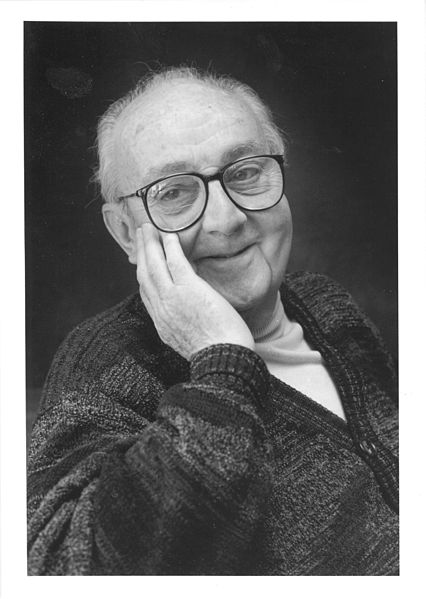
\includegraphics[width=\textwidth]{figs/Box}} \\
    \end{column}
  \end{columns}
\end{frame}




\begin{frame}
  \frametitle{Statistical models}
  \large
  {\bf What are they \alert{useful} for?}
  \begin{itemize}%[<+->]
    \item<2-> Formalizing hypotheses using math and probability
    \item[]
    \item<3-> Evaulating hypotheses by confronting models with data
    \item[]
    \item<4-> Predicting future outcomes
  \end{itemize}
\end{frame}




\begin{frame}
  \frametitle{Statistical models}
  {\bf \large Two important pieces \par}
  \large
%  \begin{enumerate}[<+- | visible@+->][\bf \color{PineGreen} (1)]
  \begin{enumerate}[\bf \color{gb} (1)]
    \large
    \item<1-> Deterministic component%(s)
      \begin{itemize}
        \large
        \item Equation for the expected value of the response
          variable %, denoted $\mathbb{E}(y)$
%        \item Often a linear model (LM), but could be a generalized
%          linear model (GLM), a generalized additive (GAM), or a
%          genearlized linear mixed effects model (GLMM), etc\dots
      \end{itemize}
    \item[]
    \item<2-> Stochastic component %(s)
      \begin{itemize}
        \large
        \item Probability distribution %(s)
          describing the differences
          between the expected values and the observed values
        \item In parametric statistics, we assume we know the
          distribution, but not the parameters of the distribution
      \end{itemize}
  \end{enumerate}
\end{frame}




%% \begin{frame}
%%   \frametitle{Example}
%%   {\bf Motivation \\}
%%   Prey numbers appear to be declining in the core of the Florida panther's range \\
%%   \pause
%%   \vfill
%%   {\bf Questions \\}
%%   How do predation, changing hydrology and hunting regulations
%%   influence white-tailed deer population viability?
%% \end{frame}


%% \begin{frame}
%%   \frametitle{Example -- South Florida Deer Study}
%% %  \begin{center}
%% %  \vspace{-8mm}
%%   \begin{columns}
%%     \begin{column}{0.6\textwidth}
%% %      \large
%%         \normalsize
%%       {\bf Objectives}
%%       \begin{enumerate}
%%         \normalsize
%%         \item[{\bf (1)}] Understand how deer populations are influenced by:
%%         \begin{itemize}
%% %          \large
%%         \normalsize
%%           \item Predation
%%           \item Hydrology
%%           \item Hunting
%%         \end{itemize}
%%         \item[{\bf (2)}] Develop a camera-based monitoring program
%%       \end{enumerate}
%%     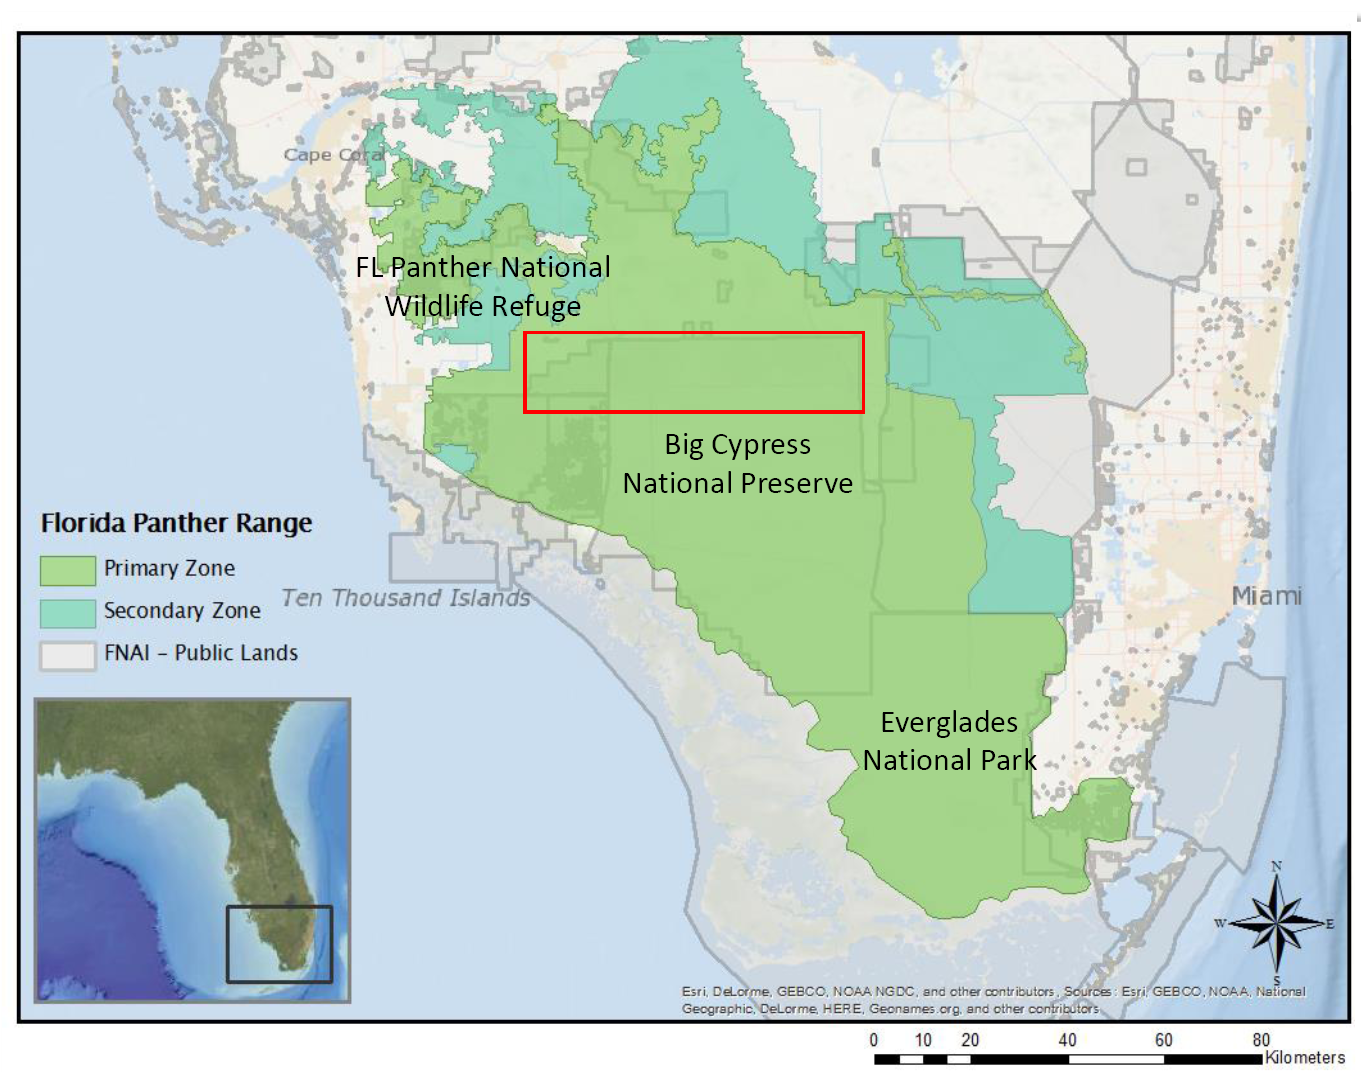
\includegraphics[width=0.9\textwidth]{figs/FL-study-area} \\ \vfill
%%     \end{column}
%%     \begin{column}{0.4\textwidth}
%%       \fbox{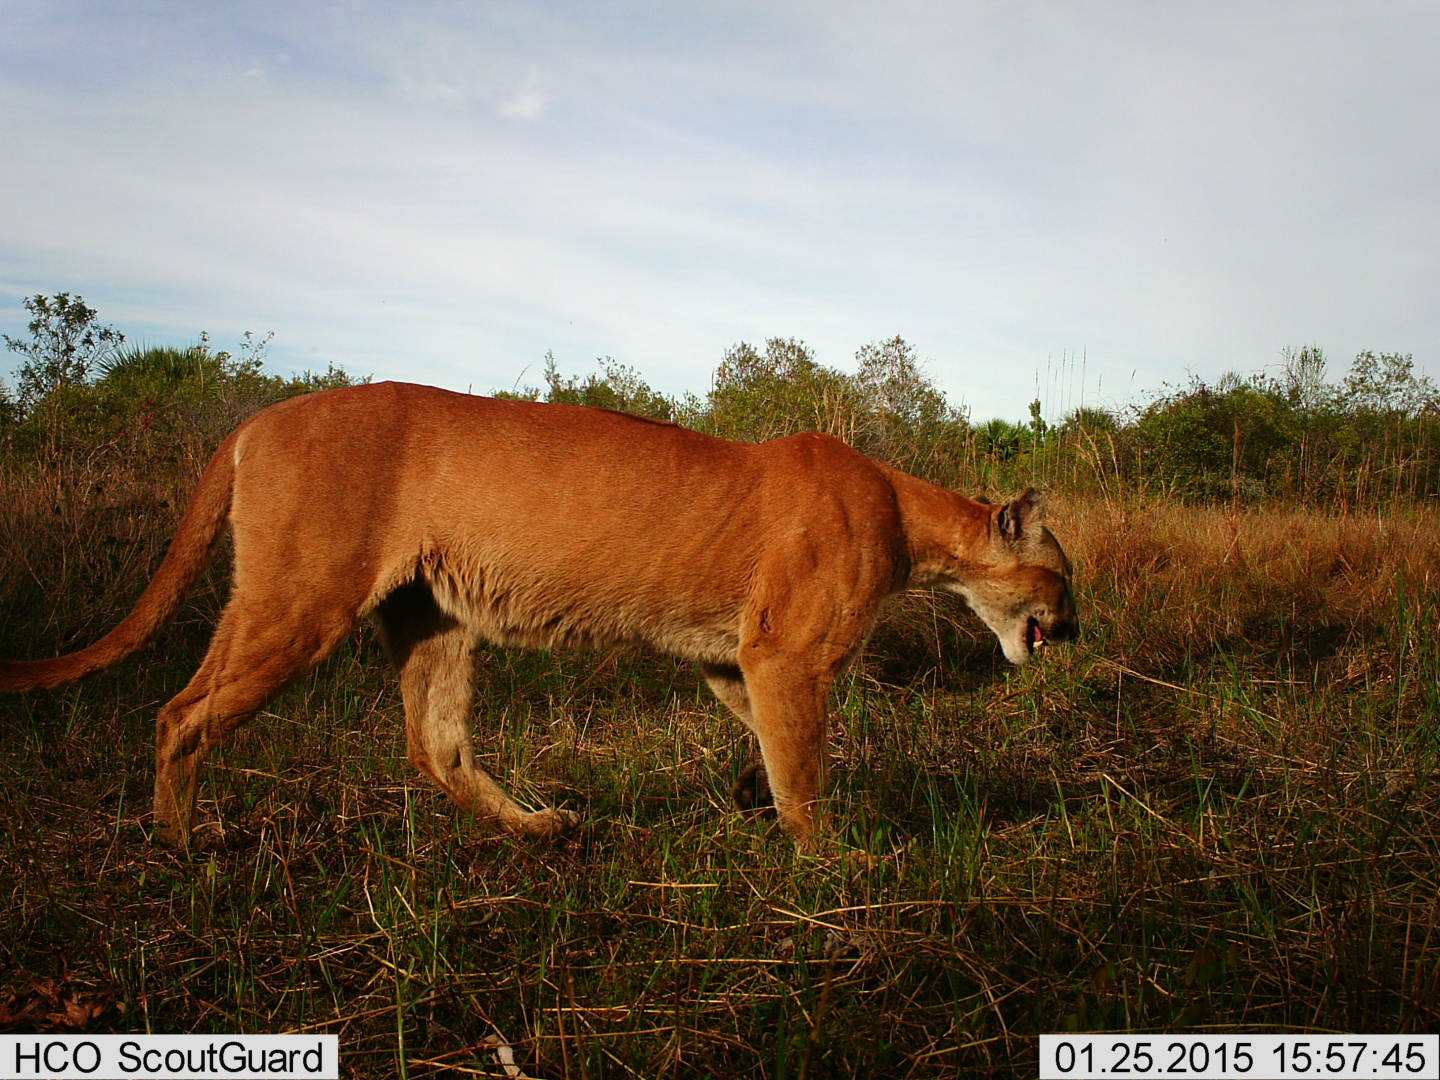
\includegraphics[width=\textwidth]{figs/puma1}} \\ \vfill
%%       \fbox{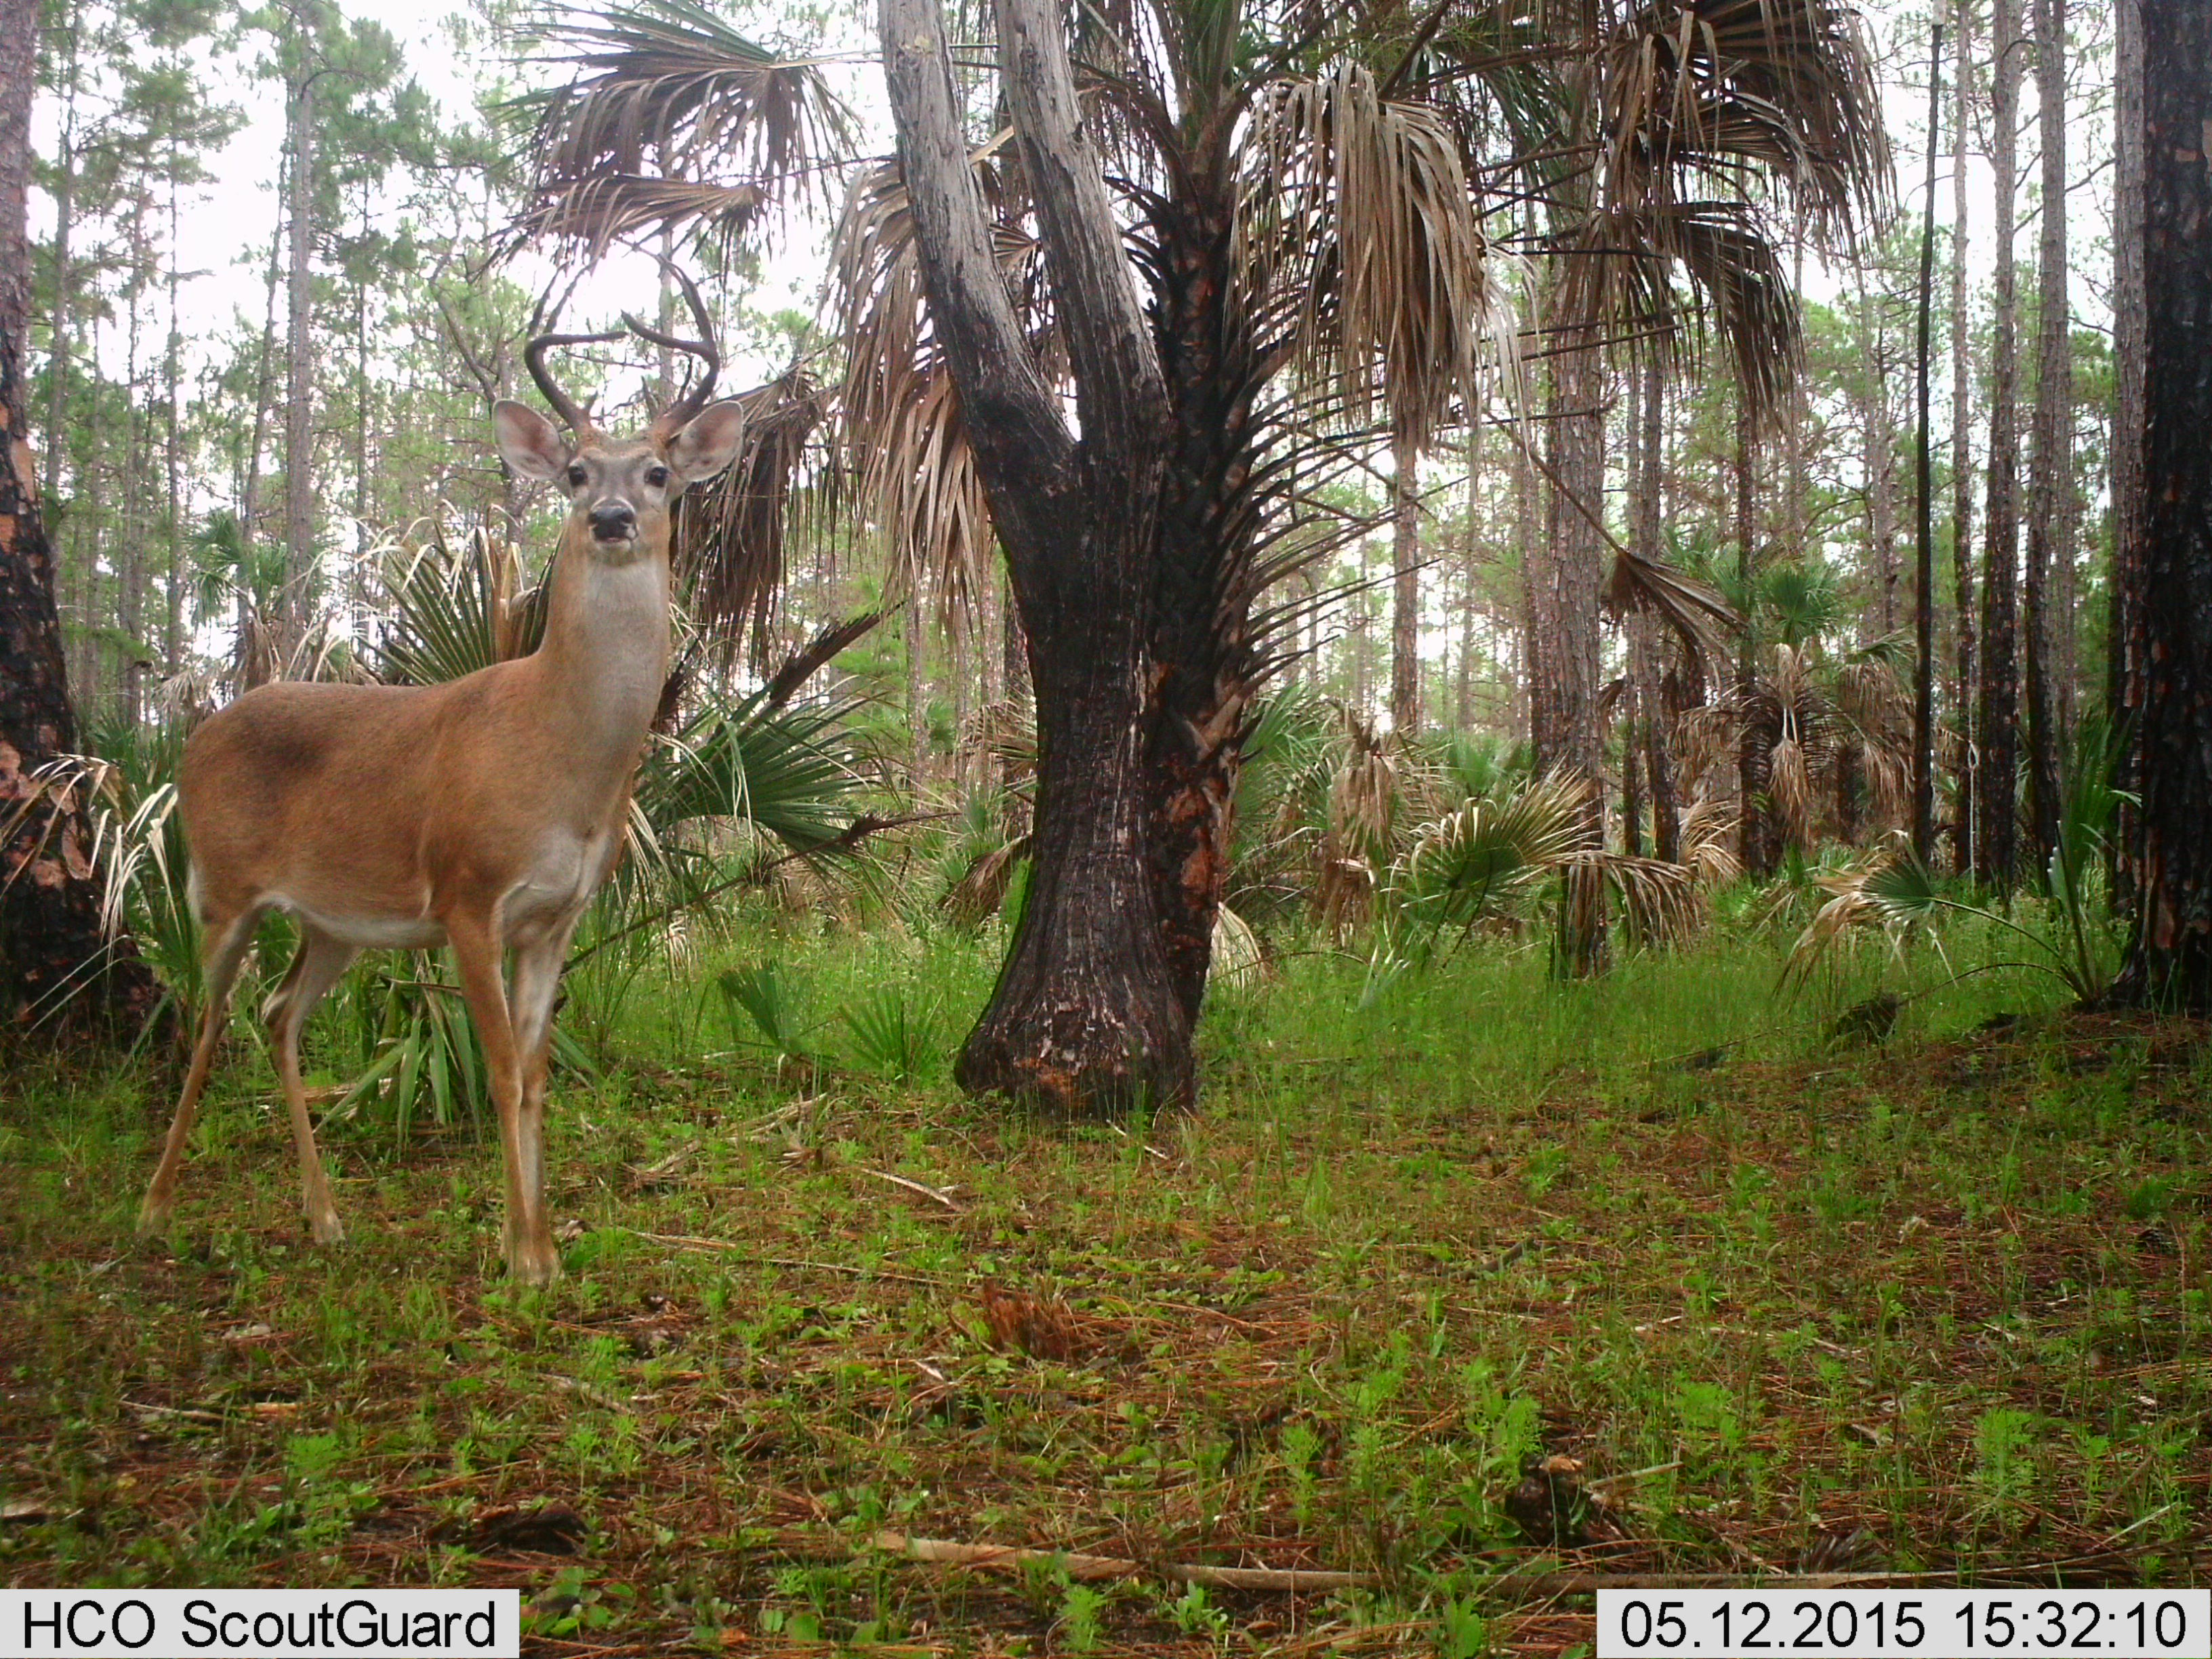
\includegraphics[width=\textwidth]{figs/2015-05-12-15-32-13_FP39}}
%%     \end{column}
%%   \end{columns}
%% %  \end{center}
%% \end{frame}









\section{Linear models}



\begin{frame}
  \frametitle{Outline}
  \LARGE
   \tableofcontents[currentsection,hideallsubsections]
\end{frame}



\begin{frame}[fragile]
  \frametitle{Is this a linear model?}
\[
y = 20 + 0.5 x
\]

\begin{center}
  \includegraphics[width=0.6\textwidth]{figure/linmod1-1}
\end{center}
\end{frame}




\begin{frame}[fragile]
  \frametitle{Is this a linear model?}
\[
y = 20 + 0.5 x - 0.3 x^2
\]

\begin{center}
  \includegraphics[width=0.6\textwidth]{figure/linmod2-1}
\end{center}
\end{frame}





\begin{frame}
  \frametitle{Linear model}
{\bf A linear model is an equation of the form:}

\[
y_i = \beta_0 + \beta_1 x_{i1} + \beta_2 x_{i2} + \ldots + \beta_p x_{ip} + \varepsilon_i
\]

where the $\beta$'s are coefficients, and the $x$ values are predictor
variables (or dummy variables for categorical predictors).
\pause

\vspace{0.5cm}

{\bf This equation is often expressed in matrix notation as:}

\[
{\bf y} = {\bf X} {\bm{\beta}} + {\bm \varepsilon}
\]

where $\bf X$ is a \alert{design matrix} and $\bm{\beta}$ is a
vector of coefficients. \pause More on matrix notation later\dots
\end{frame}


%\end{document}




\begin{frame}
  \frametitle{Interpretting the $\beta$'s}
You must be able to interpret the $\beta$
coefficients {\it for any model that you fit to your data}.
\pause
\vfill
A linear model might have dozens of continuous and categorical
predictors variables, with dozens of associated $\beta$ coefficients.
\pause
\vfill
%% Key points for interpretting $\beta$'s:
%% \begin{itemize}
%%   \item For continuous explano
%% \end{itemize}
Linear models can also include polynomial terms and interactions
between continuous and categorical predictors
\end{frame}


\begin{frame}
  \frametitle{Interpretting the $\beta$'s}% for continuous explanatory variables}
  The intercept $\beta_0$ is the expected value of $y$, when all $x$'s are 0
  \pause
  \vfill
  If $x$ is a {\bf continuous} explanatory variable: %, $\beta$ is
  \begin{itemize}
    \item $\beta$ can usually be interpretted as a \textit{slope}
      parameter.
    \item In this case, $\beta$ is the
      change in $y$ resulting from a 1 unit change in $x$ (while
      holding the other predictors constant).
  \end{itemize}
%  \pause
%  \vfill
\end{frame}




\begin{frame}[fragile]
  \frametitle{\small Interpretting $\beta$'s for categorical explantory
    variables}
  Things are more complicated for {\bf categorical} explantory
  variables (i.e., factors) because they must be converted to dummy
  variables
  \pause
  \vfill
  There are many ways of creating dummy variables
  \pause
  \vfill
%  For a {\bf categorical} explanatory variable %, $\beta$ is
  In \R, the default method for creating dummy variables from
  unordered factors works like
  this: %unordered factors is called \inr{"contr.treatment"}
  \begin{itemize}
    \item One level of the factor is treated as a \alert{reference level}
    \item The reference level is associated with the intercept
    \item The $\beta$ coefficients for the other levels of the factor
      are differences from the reference level.
  \end{itemize}
  \pause
  \vfill
  The default method corresponds to:
\begin{knitrout}\small
\definecolor{shadecolor}{rgb}{0.878, 0.918, 0.933}\color{fgcolor}\begin{kframe}
\begin{alltt}
\hlkwd{options}\hlstd{(}\hlkwc{contrasts}\hlstd{=}\hlkwd{c}\hlstd{(}\hlstr{"contr.treatment"}\hlstd{,}\hlstr{"contr.poly"}\hlstd{))}
\end{alltt}
\end{kframe}
\end{knitrout}
\end{frame}




\begin{frame}[fragile]
  \frametitle{\small Interpretting $\beta$'s for categorical explantory
    variables}
  Another common method for creating dummy variables results in
  $\beta$s that can be interpretted as the $\alpha$'s from the
  additive models that we saw earlier in the class.
  \pause
  \vfill
  With this method:
  \begin{itemize}
    \item The $\beta$ associated with each level of the factor is the
      difference from the intercept
    \item The intercept can be interpetted as the grand mean if the
      continuous variables have been centered
    \item One of the levels of the factor will not be displayed
      because it is redundant when the intercept is estimated
  \end{itemize}
  \pause
  \vfill
  This method corresponds to:
\begin{knitrout}\small
\definecolor{shadecolor}{rgb}{0.878, 0.918, 0.933}\color{fgcolor}\begin{kframe}
\begin{alltt}
\hlkwd{options}\hlstd{(}\hlkwc{contrasts}\hlstd{=}\hlkwd{c}\hlstd{(}\hlstr{"contr.sum"}\hlstd{,}\hlstr{"contr.poly"}\hlstd{))}
\end{alltt}
\end{kframe}
\end{knitrout}
\end{frame}



\section{Example}


\begin{frame}
  \frametitle{Outline}
  \LARGE
   \tableofcontents[currentsection,hideallsubsections]
\end{frame}



\begin{frame}[plain]
  \frametitle{Example}
  \Huge
  \begin{center}
    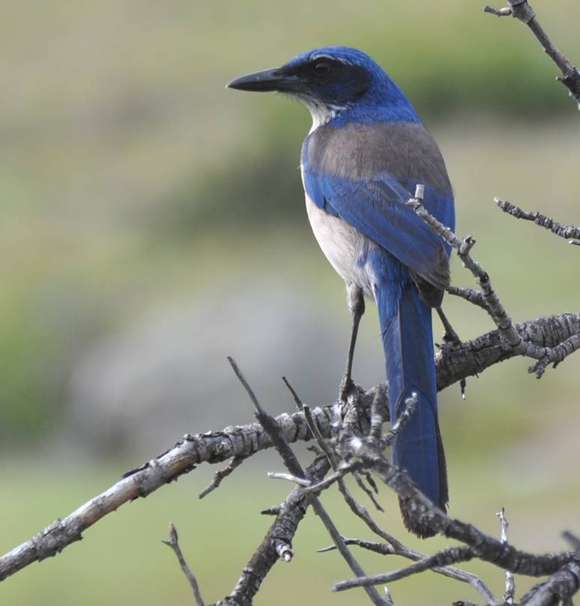
\includegraphics[width=0.5\textwidth]{figs/issj}
    The Island Scrub-Jay
  \end{center}
\end{frame}



\begin{frame}[plain]
  \frametitle{Example}
  \Huge
%  \begin{center}
  \centering
    Santa Cruz Island \\
  \begin{columns}
    \column{\dimexpr\paperwidth-20pt}
    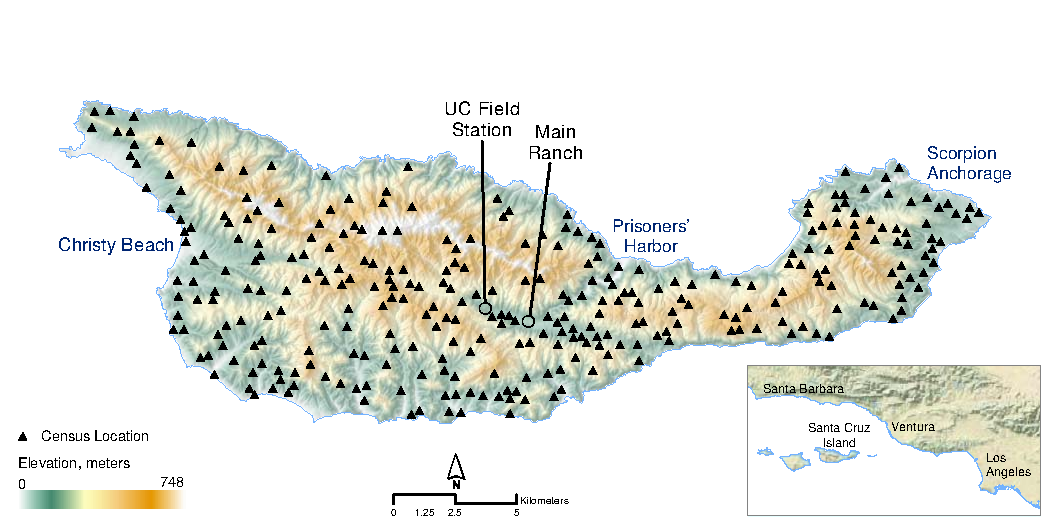
\includegraphics[width=\textwidth]{figs/Santa-Cruz} \\
  \end{columns}
%  \end{center}
\end{frame}




\begin{frame}[fragile]
  \frametitle{Santa Cruz Data}
  \footnotesize


{\bf Habitat data for all 2787 grid cells covering the island}
\begin{knitrout}
\definecolor{shadecolor}{rgb}{0.878, 0.918, 0.933}\color{fgcolor}\begin{kframe}
\begin{alltt}
\hlkwd{head}\hlstd{(cruz2)}
\end{alltt}
\begin{verbatim}
##          x       y elevation forest chaparral habitat seeds
## 1 230736.7 3774324       241      0         0     Oak   Low
## 2 231036.7 3774324       323      0         0    Pine   Med
## 3 231336.7 3774324       277      0         0    Pine  High
## 4 230436.7 3774024        13      0         0     Oak   Med
## 5 230736.7 3774024       590      0         0     Oak  High
## 6 231036.7 3774024       533      0         0     Oak   Low
\end{verbatim}
\end{kframe}
\end{knitrout}
\end{frame}



\begin{frame}[fragile]
  \frametitle{Maps of predictor variables}
%  {\bf Elevation}
  \scriptsize

\begin{columns}
  \column{\dimexpr\paperwidth-10pt}
  \includegraphics[width=\textwidth]{figure/elev-1}
\end{columns}
\end{frame}




\begin{frame}[fragile]
  \frametitle{Maps of predictor variables}
%  {\bf Forest cover}
  \scriptsize

\begin{columns}
  \column{\dimexpr\paperwidth-10pt}
  \includegraphics[width=\textwidth]{figure/forest-1}
\end{columns}
\end{frame}






\begin{frame}
  \frametitle{Questions}
  \large
%  \begin{enumerate}[<+- | visible@+->][\bf \color{PineGreen} (1)]
  \begin{enumerate}[\bf \color{PineGreen} (1)]
    \item How many jays are on the island?
    \item[]
    \item What environmental variables influence abundance?
    \item[]
    \item Can we predict consequences of environmental change?
  \end{enumerate}
\end{frame}



\begin{frame}[fragile]
  \frametitle{Maps of predictor variables}
%  {\bf Chaparral cover}

\begin{columns}
  \column{\dimexpr\paperwidth-10pt}
  \includegraphics[width=\textwidth]{figure/plots-1}
\end{columns}
\end{frame}




\begin{frame}[fragile]
  \frametitle{The (fake) jay data}
\begin{knitrout}\scriptsize
\definecolor{shadecolor}{rgb}{0.878, 0.918, 0.933}\color{fgcolor}\begin{kframe}
\begin{alltt}
\hlkwd{head}\hlstd{(jayData)}
\end{alltt}
\begin{verbatim}
##             x       y elevation forest chaparral habitat seeds jays
## 2345 258636.7 3764124       423   0.00      0.02     Oak   Med   34
## 740  261936.7 3769224       506   0.10      0.45     Oak   Med   38
## 2304 246336.7 3764124       859   0.00      0.26     Oak  High   40
## 2433 239436.7 3763524      1508   0.02      0.03    Pine   Med   43
## 1104 239436.7 3767724       483   0.26      0.37     Oak   Med   36
## 607  236436.7 3769524       830   0.00      0.01     Oak   Low   39
\end{verbatim}
\end{kframe}
\end{knitrout}
\end{frame}




\begin{frame}[fragile]
  \frametitle{Simple linear regression}
\begin{knitrout}\scriptsize
\definecolor{shadecolor}{rgb}{0.878, 0.918, 0.933}\color{fgcolor}\begin{kframe}
\begin{alltt}
\hlstd{fm1} \hlkwb{<-} \hlkwd{lm}\hlstd{(jays} \hlopt{~} \hlstd{elevation,} \hlkwc{data}\hlstd{=jayData)}
\hlkwd{summary}\hlstd{(fm1)}
\end{alltt}
\begin{verbatim}
## 
## Call:
## lm(formula = jays ~ elevation, data = jayData)
## 
## Residuals:
##     Min      1Q  Median      3Q     Max 
## -5.4874 -1.7539  0.1566  1.6159  4.6155 
## 
## Coefficients:
##              Estimate Std. Error t value Pr(>|t|)    
## (Intercept) 33.082808   0.453997   72.87   <2e-16 ***
## elevation    0.008337   0.000595   14.01   <2e-16 ***
## ---
## Signif. codes:  0 '***' 0.001 '**' 0.01 '*' 0.05 '.' 0.1 ' ' 1
## 
## Residual standard error: 2.285 on 98 degrees of freedom
## Multiple R-squared:  0.667,	Adjusted R-squared:  0.6636 
## F-statistic: 196.3 on 1 and 98 DF,  p-value: < 2.2e-16
\end{verbatim}
\end{kframe}
\end{knitrout}
\end{frame}


\begin{frame}[fragile]
  \frametitle{Simple linear regression}
\begin{knitrout}
\definecolor{shadecolor}{rgb}{0.878, 0.918, 0.933}\color{fgcolor}
\includegraphics[width=\maxwidth]{figure/pred1-1} 

\end{knitrout}
\end{frame}



\begin{frame}[fragile]
  \frametitle{Multiple linear regression}
\begin{knitrout}\scriptsize
\definecolor{shadecolor}{rgb}{0.878, 0.918, 0.933}\color{fgcolor}\begin{kframe}
\begin{alltt}
\hlstd{fm2} \hlkwb{<-} \hlkwd{lm}\hlstd{(jays} \hlopt{~} \hlstd{elevation}\hlopt{+}\hlstd{forest,} \hlkwc{data}\hlstd{=jayData)}
\hlkwd{summary}\hlstd{(fm2)}
\end{alltt}
\begin{verbatim}
## 
## Call:
## lm(formula = jays ~ elevation + forest, data = jayData)
## 
## Residuals:
##     Min      1Q  Median      3Q     Max 
## -5.4717 -1.7384  0.1552  1.5993  4.6319 
## 
## Coefficients:
##              Estimate Std. Error t value Pr(>|t|)    
## (Intercept) 33.065994   0.467624  70.711   <2e-16 ***
## elevation    0.008337   0.000598  13.943   <2e-16 ***
## forest       0.294350   1.793079   0.164     0.87    
## ---
## Signif. codes:  0 '***' 0.001 '**' 0.01 '*' 0.05 '.' 0.1 ' ' 1
## 
## Residual standard error: 2.296 on 97 degrees of freedom
## Multiple R-squared:  0.6671,	Adjusted R-squared:  0.6603 
## F-statistic: 97.21 on 2 and 97 DF,  p-value: < 2.2e-16
\end{verbatim}
\end{kframe}
\end{knitrout}
\end{frame}




\begin{frame}[fragile]
  \frametitle{Multiple linear regression}
\begin{knitrout}
\definecolor{shadecolor}{rgb}{0.878, 0.918, 0.933}\color{fgcolor}
\includegraphics[width=\maxwidth]{figure/pred2-1} 

\end{knitrout}
\end{frame}





\begin{frame}[fragile]
  \frametitle{One-way ANOVA}
\begin{knitrout}\scriptsize
\definecolor{shadecolor}{rgb}{0.878, 0.918, 0.933}\color{fgcolor}\begin{kframe}
\begin{alltt}
\hlstd{fm3} \hlkwb{<-} \hlkwd{lm}\hlstd{(jays} \hlopt{~} \hlstd{habitat,} \hlkwc{data}\hlstd{=jayData)}
\hlkwd{summary}\hlstd{(fm3)}
\end{alltt}
\begin{verbatim}
## 
## Call:
## lm(formula = jays ~ habitat, data = jayData)
## 
## Residuals:
##     Min      1Q  Median      3Q     Max 
## -7.9143 -2.3684 -0.3684  3.0857  8.6316 
## 
## Coefficients:
##             Estimate Std. Error t value Pr(>|t|)    
## (Intercept)   35.875      1.356  26.456   <2e-16 ***
## habitatOak     3.493      1.448   2.413   0.0177 *  
## habitatPine    2.039      1.503   1.357   0.1780    
## ---
## Signif. codes:  0 '***' 0.001 '**' 0.01 '*' 0.05 '.' 0.1 ' ' 1
## 
## Residual standard error: 3.835 on 97 degrees of freedom
## Multiple R-squared:  0.07126,	Adjusted R-squared:  0.05211 
## F-statistic: 3.721 on 2 and 97 DF,  p-value: 0.02773
\end{verbatim}
\end{kframe}
\end{knitrout}
\end{frame}




\begin{frame}[fragile]
  \frametitle{One-way ANOVA}

\centering
\includegraphics[width=0.8\textwidth]{figure/pred3-1} \\
\end{frame}





\begin{frame}[fragile]
  \frametitle{ANCOVA}
\begin{knitrout}\scriptsize
\definecolor{shadecolor}{rgb}{0.878, 0.918, 0.933}\color{fgcolor}\begin{kframe}
\begin{alltt}
\hlstd{fm4} \hlkwb{<-} \hlkwd{lm}\hlstd{(jays} \hlopt{~} \hlstd{elevation}\hlopt{+}\hlstd{habitat,} \hlkwc{data}\hlstd{=jayData)}
\hlkwd{summary}\hlstd{(fm4)}
\end{alltt}
\begin{verbatim}
## 
## Call:
## lm(formula = jays ~ elevation + habitat, data = jayData)
## 
## Residuals:
##     Min      1Q  Median      3Q     Max 
## -5.0327 -1.5356  0.0091  1.4686  4.2391 
## 
## Coefficients:
##              Estimate Std. Error t value Pr(>|t|)    
## (Intercept) 3.072e+01  8.084e-01  37.997  < 2e-16 ***
## elevation   8.289e-03  5.414e-04  15.308  < 2e-16 ***
## habitatOak  3.166e+00  7.850e-01   4.034  0.00011 ***
## habitatPine 1.695e+00  8.148e-01   2.081  0.04010 *  
## ---
## Signif. codes:  0 '***' 0.001 '**' 0.01 '*' 0.05 '.' 0.1 ' ' 1
## 
## Residual standard error: 2.078 on 96 degrees of freedom
## Multiple R-squared:  0.7301,	Adjusted R-squared:  0.7217 
## F-statistic: 86.56 on 3 and 96 DF,  p-value: < 2.2e-16
\end{verbatim}
\end{kframe}
\end{knitrout}
\end{frame}



\begin{frame}[fragile]
  \frametitle{ANCOVA}
\begin{knitrout}
\definecolor{shadecolor}{rgb}{0.878, 0.918, 0.933}\color{fgcolor}
\includegraphics[width=\maxwidth]{figure/pred4-1} 

\end{knitrout}
\end{frame}





\begin{frame}[fragile]
  \frametitle{Continuous-categorical interaction}
\begin{knitrout}\tiny
\definecolor{shadecolor}{rgb}{0.878, 0.918, 0.933}\color{fgcolor}\begin{kframe}
\begin{alltt}
\hlstd{fm5} \hlkwb{<-} \hlkwd{lm}\hlstd{(jays} \hlopt{~} \hlstd{elevation}\hlopt{*}\hlstd{habitat,} \hlkwc{data}\hlstd{=jayData)}
\hlkwd{summary}\hlstd{(fm5)}
\end{alltt}
\begin{verbatim}
## 
## Call:
## lm(formula = jays ~ elevation * habitat, data = jayData)
## 
## Residuals:
##    Min     1Q Median     3Q    Max 
## -5.008 -1.581 -0.103  1.420  4.184 
## 
## Coefficients:
##                        Estimate Std. Error t value Pr(>|t|)    
## (Intercept)           31.654383   1.446322  21.886  < 2e-16 ***
## elevation              0.006781   0.001999   3.393  0.00101 ** 
## habitatOak             2.428682   1.565227   1.552  0.12411    
## habitatPine            0.399953   1.579874   0.253  0.80070    
## elevation:habitatOak   0.001204   0.002153   0.559  0.57737    
## elevation:habitatPine  0.002046   0.002151   0.951  0.34414    
## ---
## Signif. codes:  0 '***' 0.001 '**' 0.01 '*' 0.05 '.' 0.1 ' ' 1
## 
## Residual standard error: 2.087 on 94 degrees of freedom
## Multiple R-squared:  0.7334,	Adjusted R-squared:  0.7192 
## F-statistic: 51.72 on 5 and 94 DF,  p-value: < 2.2e-16
\end{verbatim}
\end{kframe}
\end{knitrout}
\end{frame}




\begin{frame}[fragile]
  \frametitle{Continuous-categorical interaction}
\begin{knitrout}
\definecolor{shadecolor}{rgb}{0.878, 0.918, 0.933}\color{fgcolor}
\includegraphics[width=\maxwidth]{figure/pred5-1} 

\end{knitrout}
\end{frame}






\begin{frame}[fragile]
  \frametitle{Quadratic effect of elevation}
\begin{knitrout}\scriptsize
\definecolor{shadecolor}{rgb}{0.878, 0.918, 0.933}\color{fgcolor}\begin{kframe}
\begin{alltt}
\hlstd{fm6} \hlkwb{<-} \hlkwd{lm}\hlstd{(jays} \hlopt{~} \hlstd{elevation}\hlopt{+}\hlkwd{I}\hlstd{(elevation}\hlopt{^}\hlnum{2}\hlstd{),} \hlkwc{data}\hlstd{=jayData)}
\hlkwd{summary}\hlstd{(fm6)}
\end{alltt}
\begin{verbatim}
## 
## Call:
## lm(formula = jays ~ elevation + I(elevation^2), data = jayData)
## 
## Residuals:
##     Min      1Q  Median      3Q     Max 
## -4.8429 -1.4608  0.1304  1.5908  4.7854 
## 
## Coefficients:
##                  Estimate Std. Error t value Pr(>|t|)    
## (Intercept)     3.162e+01  7.631e-01  41.434  < 2e-16 ***
## elevation       1.368e-02  2.342e-03   5.843 6.86e-08 ***
## I(elevation^2) -3.542e-06  1.503e-06  -2.357   0.0204 *  
## ---
## Signif. codes:  0 '***' 0.001 '**' 0.01 '*' 0.05 '.' 0.1 ' ' 1
## 
## Residual standard error: 2.233 on 97 degrees of freedom
## Multiple R-squared:  0.6851,	Adjusted R-squared:  0.6786 
## F-statistic: 105.5 on 2 and 97 DF,  p-value: < 2.2e-16
\end{verbatim}
\end{kframe}
\end{knitrout}
\end{frame}




\begin{frame}[fragile]
  \frametitle{Quadratic effect of elevation}
\begin{knitrout}
\definecolor{shadecolor}{rgb}{0.878, 0.918, 0.933}\color{fgcolor}
\includegraphics[width=\maxwidth]{figure/pred6-1} 

\end{knitrout}
\end{frame}






\begin{frame}[fragile]
  \frametitle{Interaction and quadratic effects}
  \vspace{-2mm}
\begin{knitrout}\tiny
\definecolor{shadecolor}{rgb}{0.878, 0.918, 0.933}\color{fgcolor}\begin{kframe}
\begin{alltt}
\hlstd{fm7} \hlkwb{<-} \hlkwd{lm}\hlstd{(jays} \hlopt{~} \hlstd{habitat} \hlopt{*} \hlstd{forest} \hlopt{+} \hlstd{elevation} \hlopt{+}
          \hlkwd{I}\hlstd{(elevation}\hlopt{^}\hlnum{2}\hlstd{),} \hlkwc{data}\hlstd{=jayData)}
\hlkwd{summary}\hlstd{(fm7)}
\end{alltt}
\begin{verbatim}
## 
## Call:
## lm(formula = jays ~ habitat * forest + elevation + I(elevation^2), 
##     data = jayData)
## 
## Residuals:
##     Min      1Q  Median      3Q     Max 
## -5.2574 -1.4400  0.0487  1.4055  3.7924 
## 
## Coefficients:
##                      Estimate Std. Error t value Pr(>|t|)    
## (Intercept)         2.920e+01  1.030e+00  28.338  < 2e-16 ***
## habitatOak          3.705e+00  8.433e-01   4.394 2.98e-05 ***
## habitatPine         2.216e+00  8.757e-01   2.531   0.0131 *  
## forest              4.007e+01  2.780e+01   1.441   0.1529    
## elevation           1.215e-02  2.300e-03   5.285 8.41e-07 ***
## I(elevation^2)     -2.554e-06  1.484e-06  -1.721   0.0886 .  
## habitatOak:forest  -4.292e+01  2.785e+01  -1.541   0.1267    
## habitatPine:forest -3.918e+01  2.784e+01  -1.407   0.1627    
## ---
## Signif. codes:  0 '***' 0.001 '**' 0.01 '*' 0.05 '.' 0.1 ' ' 1
## 
## Residual standard error: 2.044 on 92 degrees of freedom
## Multiple R-squared:  0.7497,	Adjusted R-squared:  0.7307 
## F-statistic: 39.37 on 7 and 92 DF,  p-value: < 2.2e-16
\end{verbatim}
\end{kframe}
\end{knitrout}
\end{frame}



\begin{frame}[fragile]
  \frametitle{Predict jay abundance at each grid cell}
\begin{knitrout}
\definecolor{shadecolor}{rgb}{0.878, 0.918, 0.933}\color{fgcolor}\begin{kframe}
\begin{alltt}
\hlstd{E7} \hlkwb{<-} \hlkwd{predict}\hlstd{(fm7,} \hlkwc{type}\hlstd{=}\hlstr{"response"}\hlstd{,} \hlkwc{newdata}\hlstd{=cruz2,}
              \hlkwc{interval}\hlstd{=}\hlstr{"confidence"}\hlstd{)}
\end{alltt}
\end{kframe}
\end{knitrout}
\pause
\begin{knitrout}
\definecolor{shadecolor}{rgb}{0.878, 0.918, 0.933}\color{fgcolor}\begin{kframe}
\begin{alltt}
\hlstd{E7} \hlkwb{<-} \hlkwd{cbind}\hlstd{(cruz2[,}\hlkwd{c}\hlstd{(}\hlstr{"x"}\hlstd{,}\hlstr{"y"}\hlstd{)], E7)}
\hlkwd{head}\hlstd{(E7)}
\end{alltt}
\begin{verbatim}
##          x       y      fit      lwr      upr
## 1 230736.7 3774324 35.68349 34.86313 36.50386
## 2 231036.7 3774324 35.07284 34.22917 35.91652
## 3 231336.7 3774324 34.58427 33.72668 35.44186
## 4 230436.7 3774024 33.06042 31.55907 34.56177
## 5 230736.7 3774024 39.18440 38.49766 39.87113
## 6 231036.7 3774024 38.65512 37.98859 39.32165
\end{verbatim}
\end{kframe}
\end{knitrout}
\end{frame}


\begin{frame}[fragile]
  \frametitle{Map the predictions}
  \scriptsize

\begin{columns}
  \column{\dimexpr\paperwidth-10pt}
  \includegraphics[width=\textwidth]{figure/Ejay-1}
\end{columns}
\end{frame}




\begin{frame}[fragile]
  \frametitle{Map the predictions}
  \scriptsize

\begin{columns}
  \column{\dimexpr\paperwidth-10pt}
  \includegraphics[width=\textwidth]{figure/Ljay-1}
\end{columns}
\end{frame}




\begin{frame}[fragile]
  \frametitle{Map the predictions}
  \scriptsize

\begin{columns}
  \column{\dimexpr\paperwidth-10pt}
  \includegraphics[width=\textwidth]{figure/Ujay-1}
\end{columns}
\end{frame}




%% \begin{frame}[fragile]
%%   \frametitle{Future scenarios}
%%   {\bf What if the pine and oak disappear? \par}
%%   \pause
%%   \vspace{0.3cm}
%%   {\bf \dots assuming {\tt fm5} is the {\it correct} model}
%%   \pause
%%   \vspace{0.3cm}
%%   \footnotesize
%% <<>>=
%% future1 <- cruz2
%% future1$habitat[] <- "Bare"
%% future.pred1 <- predict(fm5, type="response", newdata=future1,
%%                         interval="confidence")
%% future.pred1 <- cbind(cruz2[,c("x","y")], future.pred1)
%% @
%% \end{frame}



\begin{frame}[fragile]
  \frametitle{Future scenarios}
  {\bf What if pine and oak disapper? \par}
  \scriptsize


\begin{columns}
  \column{\dimexpr\paperwidth-10pt}
  \only<1>{\includegraphics[width=\textwidth]{figure/Ejay-1} \\}
  \only<2>{\includegraphics[width=\textwidth]{figure/future1fig-1} \\}
\end{columns}
\end{frame}





%% \begin{frame}[fragile]
%%   \frametitle{Future scenarios}
%%   {\bf What if the island sinks 1000 m? \par}
%%   \vspace{0.3cm}
%% %  \pause
%% %  {\bf \dots assuming {\tt fm5} is the {\it correct} model}
%%   \pause
%%   \footnotesize
%% <<>>=
%% future2 <- cruz2
%% future2$elevation <- future2$elevation - 1000
%% future2$elevation[future2$elevation < 0] <- NA
%% future.pred2 <- predict(fm5, type="response", newdata=future2,
%%                         interval="confidence")
%% future.pred2 <- cbind(cruz2[,c("x","y")], future.pred2)
%% @
%% \end{frame}




\begin{frame}[fragile]
  \frametitle{Future scenarios}
  {\bf What if sea level rises? \par}
  \scriptsize
  \pause


\begin{columns}
  \column{\dimexpr\paperwidth-10pt}
  \includegraphics[width=\textwidth]{figure/future2fig-1}
\end{columns}
\end{frame}



%% \begin{frame}
%%   \frametitle{Worse yet \dots}
%%   \pause
%%   \huge
%%   What if our model is wrong?
%% \end{frame}












\section{Matrix notation}


\begin{frame}
  \frametitle{Outline}
  \LARGE
   \tableofcontents[currentsection,hideallsubsections]
\end{frame}



\begin{frame}
  \frametitle{Matrix notation}
  Linear models are often expressed in matrix notation \\
  \vfill
  There are two reasons for this: \\
  \begin{itemize}%[(1)]
    \item It is more compact and therefore easier to write
    \item Matrix multiplication is fast on a computer
  \end{itemize}
\end{frame}



\begin{frame}
  \frametitle{Linear model}
  {\bf All of the fixed effects models that we have covered can be
    expressed this way:}
  \[
  {\bf y} = {\bf X}{\bm \beta} + {\bm \varepsilon}
  \]
  {\bf where}
  \[
  {\bm \varepsilon} \sim \mbox{Normal}(0, \sigma^2)
  \]
  \pause
  \vfill
  {\bf Examples include} \\
  \begin{itemize}
    \item Completely randomized ANOVA
    \item Randomized complete block designs with fixed block effects
    \item Factorial designs
    \item ANCOVA
  \end{itemize}
\end{frame}






\begin{frame}
  \frametitle{Then how do they differ?}
%  \pause
  \begin{itemize}%[<+->]
  \large
    \item The design matrices are different
    \item[]
    \item And so are the number of parameters (coefficients) to be
      estimated
    \item[]
    \item Important to understand how to construct design matrix that
      includes categorical variables
  \end{itemize}
\end{frame}




\begin{frame}%[fragile]
  \frametitle{Design matrix}
%  \large
%  \begin{itemize}[<+->]
%    \item
  A design matrix has $N$ rows and $K$ columns, where $N$ is
      the total sample size and $K$ is the number of coefficients (parameters)
      to be estimated. \\
 \pause
 \vfill
%    \item
      The first column contains just 1's. This column corresponds
      to the intercept ($\beta_0$) \\
 \pause
 \vfill
%    \item
      Continuous predictor variables appear unchanged in the design
      matrix \\
 \pause
 \vfill
%    \item
      Categorical predictor variables appear as dummy variables \\
 \pause
 \vfill
%    \item
      In {\bf R}, the design matrix is created internally based on
      the formula that you provide \\
 \pause
 \vfill
%    \item
      The design matrix can be viewed using the \inr{model.matrix} function
%  \end{itemize}
\end{frame}





%% \begin{frame}[fragile]
%%   \frametitle{Design matrix for linear regression}
%%   \begin{columns}
%%     \begin{column}{0.5\textwidth}
%%     {\bf Data}
%%       \scriptsize %\tiny
%% %<<>>=
%% %options(digits=2)
%% %@
%% <<dietData,size='scriptsize'>>=
%% dietData <- read.csv("dietData.csv")
%% head(dietData, n=10)
%% @
%%     \end{column}
%%     \pause
%%     \begin{column}{0.5\textwidth}
%%       {\bf Design matrix}
%%       \scriptsize %\tiny
%% <<X1,size='scriptsize'>>=
%% X1 <- model.matrix(~age,
%%                    data=dietData)
%% head(X1, n=10)
%% @
%%     \end{column}
%%   \end{columns}
%%   \pause
%%   \vfill
%%   {\centering \bf How do we multiply this design matrix ($\bf X$) by
%%     the vector of regression coefficients ($\bm \beta$)? \par}
%% \end{frame}








\begin{frame}[fragile]
  \frametitle{Design matrix for linear regression}
%  \begin{columns}
%    \begin{column}{0.5\textwidth}
  \scriptsize %\tiny
    {Model}
\begin{knitrout}\scriptsize
\definecolor{shadecolor}{rgb}{0.878, 0.918, 0.933}\color{fgcolor}\begin{kframe}
\begin{alltt}
\hlstd{fm1} \hlkwb{<-} \hlkwd{lm}\hlstd{(jays} \hlopt{~} \hlstd{elevation,} \hlkwc{data}\hlstd{=jayData)}
\end{alltt}
\end{kframe}
\end{knitrout}
%    \end{column}
    \pause
    \vfill
%    \begin{column}{0.5\textwidth}
      {Design matrix}
      \scriptsize %\tiny
\begin{knitrout}\scriptsize
\definecolor{shadecolor}{rgb}{0.878, 0.918, 0.933}\color{fgcolor}\begin{kframe}
\begin{alltt}
\hlstd{X1} \hlkwb{<-} \hlkwd{model.matrix}\hlstd{(fm1)}
\hlkwd{head}\hlstd{(X1,} \hlkwc{n}\hlstd{=}\hlnum{5}\hlstd{)} \hlcom{# First 5 rows of design matrix}
\end{alltt}
\begin{verbatim}
##      (Intercept) elevation
## 2345           1       423
## 740            1       506
## 2304           1       859
## 2433           1      1508
## 1104           1       483
\end{verbatim}
\end{kframe}
\end{knitrout}
%    \end{column}
%  \end{columns}
      {Estimated $\beta$ coefficients}
      \scriptsize %\tiny
\begin{knitrout}\scriptsize
\definecolor{shadecolor}{rgb}{0.878, 0.918, 0.933}\color{fgcolor}\begin{kframe}
\begin{alltt}
\hlstd{beta.hat} \hlkwb{<-} \hlkwd{coef}\hlstd{(fm1)} \hlcom{# Estimates of beta0 and beta1}
\hlstd{beta.hat}
\end{alltt}
\begin{verbatim}
##  (Intercept)    elevation 
## 33.082808066  0.008336657
\end{verbatim}
\end{kframe}
\end{knitrout}
  \pause
  \vfill
  {\centering How do we multiply the design matrix ($\bf X$) by
    the vector of regression coefficients ($\bm \beta$)? \\}
\end{frame}








\begin{frame}
  \frametitle{Matrix multiplication}
  \Large
  \begin{center}
    \[
      \mathbb{E}({\bf y}) = {\bf X}{\bm \beta}
    \]
    \[
    \uncover<3->{
    \begin{bmatrix}
      aw + bx + cy + dz \\
      ew + fx + gy + hz \\
      iw + jx + ky + lz %\\
%      mw + nx + oy + pz
    \end{bmatrix}
    }
    \uncover<2->{=}
    \uncover<2->{
    \begin{bmatrix}
      a & b & c & d \\
      e & f & g & h \\
      i & j & k & l %\\
%      m & n & o & p
    \end{bmatrix}
    }
    \uncover<2->{
    \times
    \begin{bmatrix}
      w \\
      x \\
      y \\
      z
    \end{bmatrix}
    }
    \]
  \end{center}
  \normalsize
  \uncover<4->{
    {\bf In this example}}
    \begin{itemize}
      \item<4-> The first matrix corresponds to the expected values of $\bm y$
      \item<4-> The second matrix corresponds to the design matrix {$\bf X$}
      \item<4-> The third matrix corresponds to {$\bm \beta$}
    \end{itemize}
\end{frame}






\begin{frame}[fragile]
  \frametitle{Matrix multiplication}
%% {\bf \centering The vector of coefficients \\}
%% %\small
%% <<beta,size='small'>>=
%% beta <- coef(fm1)
%% beta
%% @
%% \pause
%\large
\begin{center}
  {$\mathbb{E}({\bf y}) = {\bf X}{\bm \beta}$ or $\mathbb{E}(y_i) = \beta_0 + \beta_1 \mathrm{ELEV}_i$}
\end{center}
\pause
\small
\begin{knitrout}\footnotesize
\definecolor{shadecolor}{rgb}{0.878, 0.918, 0.933}\color{fgcolor}\begin{kframe}
\begin{alltt}
\hlstd{Ey1} \hlkwb{<-} \hlstd{X1} \hlopt \hlstd{beta.hat} \hlcom{# Expected number of jays at each site}
\hlkwd{head}\hlstd{(Ey1,} \hlnum{5}\hlstd{)}
\end{alltt}
\begin{verbatim}
##          [,1]
## 2345 36.60921
## 740  37.30116
## 2304 40.24400
## 2433 45.65449
## 1104 37.10941
\end{verbatim}
\end{kframe}
\end{knitrout}
\end{frame}









\begin{frame}[fragile]
  \frametitle{Design matrix for ANCOVA}
  \scriptsize %\tiny
    {Model}
\begin{knitrout}\scriptsize
\definecolor{shadecolor}{rgb}{0.878, 0.918, 0.933}\color{fgcolor}\begin{kframe}
\begin{alltt}
\hlstd{fm4} \hlkwb{<-} \hlkwd{lm}\hlstd{(jays} \hlopt{~} \hlstd{elevation} \hlopt{+} \hlstd{habitat,} \hlkwc{data}\hlstd{=jayData)}
\end{alltt}
\end{kframe}
\end{knitrout}
\pause
\vfill
{Design matrix}

\begin{knitrout}\scriptsize
\definecolor{shadecolor}{rgb}{0.878, 0.918, 0.933}\color{fgcolor}\begin{kframe}
\begin{alltt}
\hlstd{X4} \hlkwb{<-} \hlkwd{model.matrix}\hlstd{(fm4)}
\hlkwd{head}\hlstd{(X4,} \hlkwc{n}\hlstd{=}\hlnum{5}\hlstd{)} \hlcom{# First 5 rows of design matrix}
\end{alltt}
\begin{verbatim}
##      (Intercept) elevation habitatOak habitatPine
## 2345           1       423          1           0
## 740            1       506          1           0
## 2304           1       859          1           0
## 2433           1      1508          0           1
## 1104           1       483          1           0
\end{verbatim}
\end{kframe}
\end{knitrout}

{Estimated $\beta$ coefficients}
\begin{knitrout}\scriptsize
\definecolor{shadecolor}{rgb}{0.878, 0.918, 0.933}\color{fgcolor}\begin{kframe}
\begin{alltt}
\hlstd{beta.hat4} \hlkwb{<-} \hlkwd{coef}\hlstd{(fm4)} \hlcom{# Estimates of beta0 and beta1}
\hlstd{beta.hat4}
\end{alltt}
\begin{verbatim}
##  (Intercept)    elevation   habitatOak  habitatPine 
## 30.716371786  0.008288617  3.166147905  1.695456106
\end{verbatim}
\end{kframe}
\end{knitrout}
\pause
\vfill
{\centering How do we multiply the design matrix ($\bf X$) by
 the vector of regression coefficients ($\bm \beta$)? \\}
\end{frame}




\begin{frame}[fragile]
  \frametitle{Matrix multiplication}
\begin{center}
  \small
  {$\mathbb{E}({\bf y}) = {\bf X}{\bm \beta}$ or $\mathbb{E}(y_i) = \beta_0 +
    \beta_1 \mathrm{ELEV}_i + \beta_2 \mathrm{OAK}_i + \beta_3 \mathrm{PINE}_i$}
\end{center}
\pause
\small
\begin{knitrout}\footnotesize
\definecolor{shadecolor}{rgb}{0.878, 0.918, 0.933}\color{fgcolor}\begin{kframe}
\begin{alltt}
\hlstd{Ey4} \hlkwb{<-} \hlstd{X4} \hlopt \hlstd{beta.hat4} \hlcom{# Expected number of jays at each site}
\hlkwd{head}\hlstd{(Ey4,} \hlnum{5}\hlstd{)}
\end{alltt}
\begin{verbatim}
##          [,1]
## 2345 37.38860
## 740  38.07656
## 2304 41.00244
## 2433 44.91106
## 1104 37.88592
\end{verbatim}
\end{kframe}
\end{knitrout}
\end{frame}










\begin{frame}
  \frametitle{Summary}
  Linear models are the foundation of modern statistical modeling
  techniques \\
  \pause
  \vfill
  They can be used to model a wide array of biological processes, and
  they can be easily extended when their assumptions do not hold \\
  \pause
  \vfill
  One of the most important extensions is to cases where the residuals
  are not normally distributed. Generalized linear models address this
  issue.
\end{frame}





%\subsection{Distributions}




%\subsection{Fixed effects models}



%% \begin{frame}
%%   \frametitle{Linear regression}
%% {\bf Deterministic part:}
%% %\[
%% %\mu_i = \mathbb{E}(\bf y) = \beta_0 + \beta_1x_i
%% %\]
%% %\pause
%% %{\bf The same thing, using matrix notation:}
%% \[
%% {\bm \mu} = \mathbb{E}(\bf y) = {\bf X}{\bm \beta}
%% \]
%% \pause
%% {\bf Stochastic part:}
%% %\[
%% %y_i \sim \mbox{Normal}(\mu_i, \sigma^2)
%% %\]
%% %\pause
%% %\centering or \par
%% \[
%% \varepsilon_i \sim \mbox{Normal}(0, \sigma^2)
%% \]
%% \end{frame}




%% \begin{frame}
%%   \frametitle{One-way ANOVA}
%% {\bf Deterministic part:}
%% \[
%% {\bm \mu} = \mathbb{E}(\bf y) = {\bf X}{\bm \beta}
%% \]
%% {\bf Stochastic part:}
%% %\[
%% %y_i \sim \mbox{Normal}(\mu_i, \sigma^2)
%% %\]
%% \[
%% \varepsilon_i \sim \mbox{Normal}(0, \sigma^2)
%% \]
%% \end{frame}




%% \begin{frame}
%%   \frametitle{A$\times$B Factorial ANOVA}
%% {\bf Deterministic part:}
%% \[
%% {\bm \mu} = \mathbb{E}(\bf y) = {\bf X}{\bm \beta}
%% \]
%% {\bf Stochastic part:}
%% %\[
%% %y_i \sim \mbox{Normal}(\mu_i, \sigma^2)
%% %\]
%% \[
%% \varepsilon_i \sim \mbox{Normal}(0, \sigma^2)
%% \]
%% \end{frame}



%% \begin{frame}
%%   \frametitle{A$\times$B$\times$C Factorial ANOVA}
%% {\bf Deterministic part:}
%% \[
%% {\bm \mu} = \mathbb{E}(\bf y) = {\bf X}{\bm \beta}
%% \]
%% {\bf Stochastic part:}
%% %\[
%% %y_i \sim \mbox{Normal}(\mu_i, \sigma^2)
%% %\]
%% \[
%% \varepsilon_i \sim \mbox{Normal}(0, \sigma^2)
%% \]
%% \end{frame}



%% \begin{frame}
%%   \frametitle{ANCOVA}
%% {\bf Deterministic part:}
%% \[
%% {\bm \mu} = \mathbb{E}(\bf y) = {\bf X}{\bm \beta}
%% \]
%% {\bf Stochastic part:}
%% %\[
%% %y_i \sim \mbox{Normal}(\mu_i, \sigma^2)
%% %\]
%% \[
%% \varepsilon_i \sim \mbox{Normal}(0, \sigma^2)
%% \]
%% \end{frame}



%% \begin{frame}
%%   \frametitle{Another equivalent expression}
%%   {\bf General linear model}
%%   \[
%%   {\bf y} = {\bf X}{\bm \beta} + {\bm \epsilon}
%%   \]
%%   {\bf where}
%%   \[
%%   {\bm \epsilon} \sim \mbox{Normal}(0, {\bf I}\sigma^2)
%%   \]
%% \end{frame}





% \begin{frame}[fragile]
%   \frametitle{One-way ANOVA}
%   \scriptsize %\tiny
% <<lm2,size='scriptsize'>>=
% lm2 <- lm(weight ~ diet, data=dietData)
% summary(lm2)
% @
% \end{frame}



% \begin{frame}[fragile]
%   \frametitle{One-way ANOVA: Design matrix}
% <<X2>>=
% X2 <- model.matrix(~diet, data=dietData)
% X2[20:30,]
% @
% \end{frame}


% \begin{frame}[fragile]
%   \frametitle{One-way ANOVA: Expected values of $y$}
%   \footnotesize %\scriptsize
% <<betas2,size='footnotesize'>>=
% betas2 <- coef(lm2)
% betas2
% @
% \pause
% <<Ey2,size='footnotesize'>>=
% Ey2 <- X2 %*% betas2
% head(Ey2)
% @
% \end{frame}



% \begin{frame}[fragile]
%   \frametitle{ANCOVA}
%   \vspace{-2mm}
%   \scriptsize %\tiny
% <<lm3,size='scriptsize'>>=
% lm3 <- lm(weight ~ age + diet, data=dietData)
% summary(lm3)
% @
% \end{frame}



% \begin{frame}[fragile]
%   \frametitle{ANCOVA: Design matrix}
% <<X3>>=
% X3 <- model.matrix(~age+diet, data=dietData)
% X3[20:30,]
% @
% \end{frame}




% \begin{frame}[fragile]
%   \frametitle{ANCOVA: Expected values of $y$}
%   \footnotesize
% <<betas3,size='footnotesize'>>=
% betas3 <- coef(lm3)
% betas3
% @
% <<Ey3,size='footnotesize'>>=
% Ey3 <- X3 %*% betas3
% head(Ey3)
% @
% \end{frame}



% \begin{frame}[fragile]
%   \frametitle{Beyond ANCOVA}
%   {\bf Now the slopes differ for each treatment}
%   \tiny
% <<lm4,size='tiny'>>=
% lm4 <- lm(weight ~ diet * age, data=dietData)
% summary(lm4)
% @
% \end{frame}




% \begin{frame}[fragile]
%   \frametitle{The associated design matrix}
%   \tiny
% <<X4,size='tiny'>>=
% X4 <- model.matrix(~ diet * age, data=dietData)
% X4[20:30,]
% @
% \pause
% <<betas4>>=
% betas4 <- coef(lm4)
% Ey4 <- X4 %*% betas4
% @
% \end{frame}





%% \begin{frame}[fragile]
%%   \frametitle{Beyond ANCOVA}
%%   {\bf ... and we test for a moon effect}
%%   \tiny
%% <<>>=
%% lm3 <- lm(weight ~ diet * age + moon, data=dietData)
%% summary(lm3)
%% @
%% \end{frame}


%% \begin{frame}
%%   \frametitle{Mixed effects models}
%% {\bf The notation is only slightly more complex}
%% \end{frame}



%\subsection{Mixed effects models}









\end{document}

